\section{Making a Monte Carlo integrator}


First, we explored different methods
in order to gain a better insight on how to create a better general integrator. We tested 4 methods, where each differs in how
the points in the domain are chosen to evaluate the integral.
The integration schemes \cite{MCmethods} used are, figure \ref{BoxPlotter} shows
the point distribution for the domian in each method:
\begin{enumerate}
  \item Uniform Static - The entire domain is divided by a uniform mesh were each point is taken in a coordinate is the grid.
  \item Uniform Adaptive - The domain is divided uniformly in square boxes, and for each box a mesh grid is created
  specified by a density value which determines the total number of points inside that box. The density parameter
  is obtained by performing successive iterations, on which the density of each sub-box is set by the total value of the integral inside
  the box.
  \item Stratified Static - The entire domain is divided in a uniform mesh, where for each quadrant of the mesh
  a single point is chosen randomly inside.
  \item Stratified Adaptive - A combination of both methods adaptive and stratified.
\end{enumerate}
\begin{figure*}
  \begin{center}
    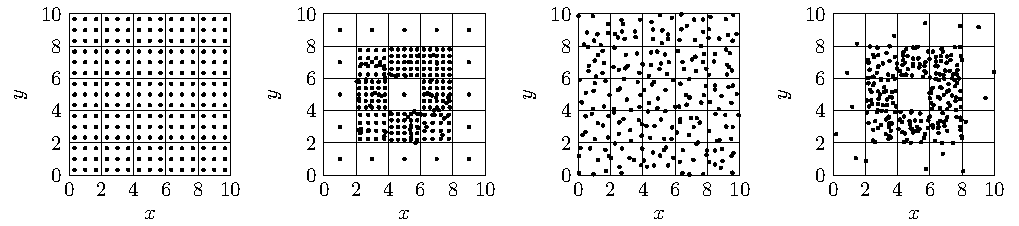
\includegraphics[scale=1 ]{graphs/BoxPlotter.pdf}
  \caption{Illustrative examples of (from left to right) a uniform static, uniform adaptive, stratified static and stratified adaptive integration schemes. The lines create boxes within which an internal grid is applied in the case of static integration schemes. Notice that in all cases the number of points is the same, which in the case of adaptive static causes us to end with some points which do not fit in a grid. To accommodate for this we distributed them randomly within their respective box. }
\label{BoxPlotter}
  \end{center}
\end{figure*}

To compare each method we used a test function on which we evaluated the integrals.
This test function consisted of a ring with constant value in a 2-dimensional domain as seen in fig. \ref{BoxPlotter}, from which
we can know the exact value of the integral easily. The results
of the error obtained for the different methods as a function of the number of points used is shown in fig. \ref{MCerrs},
 where 500 repetitions where used for each number of points and in the case of adaptive methods the entire integration
 domain was divided into 25 boxes. As
expected the best method is the adaptive stratified which has also gives the smallest standard deviation from the error as seen in the error bars (Where
the uniform static is an exception, since the points are always fixed there is no error to report).
Additionally it is important to note how the error of the uniform static method, and in lesser degree in the adaptive static,
 increases at some point as the number of points increases, this systematic error introduced by the regular mesh. This shows the entire point of doing Monte Carlo integration!
\begin{figure*}[ht]
  \begin{center}
  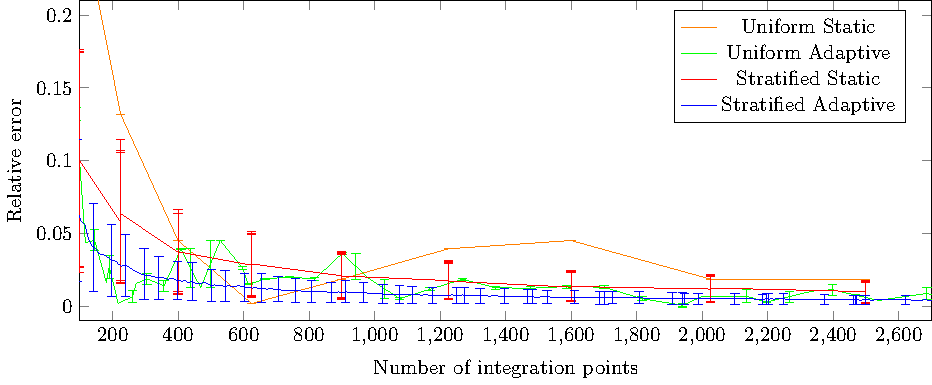
\includegraphics[scale=1 ]{graphs/integration_test_ring.pdf}
  \caption{Performance comparison of different numeric integration methods. The absolute value of the difference between the numerically calculated result and the analytical answer plotted against the number of integration points used. The used function is a two-dimensional ring (see text).}
  \label{MCerrs}
  \end{center}
\end{figure*}

Now that we know the best method is the adaptive stratified, we will use it through the rest of this work to solve every integral neded.
